\documentclass[12pt]{article}
\usepackage[margin=1.2in]{geometry}
\usepackage[all]{nowidow}
\usepackage[hyperfigures=true, hidelinks, pdfhighlight=/N]{hyperref}
\usepackage{graphicx,amsmath,physics,tabto,float,amssymb,pgfplots,verbatim,tcolorbox}
\usepackage{listings,xcolor,siunitx,subfig,keyval2e,caption,import}
\numberwithin{equation}{section}
\numberwithin{figure}{section}
\definecolor{stringcolor}{HTML}{C792EA}
\definecolor{codeblue}{HTML}{2162DB}
\definecolor{commentcolor}{HTML}{4A6E46}
\lstdefinestyle{appendix}{
    basicstyle=\ttfamily\footnotesize,commentstyle=\color{commentcolor},keywordstyle=\color{codeblue},
    stringstyle=\color{stringcolor},showstringspaces=false,numbers=left,upquote=true,captionpos=t,
    abovecaptionskip=12pt,belowcaptionskip=12pt,language=Python,breaklines=true,frame=single}
\lstdefinestyle{inline}{
    basicstyle=\ttfamily\footnotesize,commentstyle=\color{commentcolor},keywordstyle=\color{codeblue},
    stringstyle=\color{stringcolor},showstringspaces=false,numbers=left,upquote=true,frame=tb,
    captionpos=b,language=Python}
\renewcommand{\lstlistingname}{Appendix}
\pgfplotsset{compat=1.17}

\title{LRC Circuit}
\date{\textbf{1 September 2020}}
\author{KDSMIL001 \; PHY2004W}

\begin{document}
    \begin{titlepage}
        \maketitle
        \center
        \tableofcontents
    \end{titlepage}
    
    \section{Introduction}\label{sec:Introduction}
    In this report we will investigate the LRC circuit in two different forms; the parallel resonant 
    circuit and the series resonant circuit. More on what those are a bit later. For now we just need 
    to know that an LRC circuit is comprised of an inductor (L), a resistor (R), and a capacitor(C), 
    as well as some kind of applied voltage. In this experiment we will be using an alternating voltage 
    as it results in some interesting behaviours. We will get into these behaviours more in later 
    sections but for now all we need to know is that any kind of LRC circuit will have a resonant 
    driving frequency at which the current (and thus the voltage) as well as the impedance in the 
    circuit will be at an extremum. In order to see how each configuration will behave, let's 
    investigate them analytically first.

    \section{The Parallel Resonance LRC Circuit}\label{sec:Parallel Resonance}
    The parallel resonance set-up for an LRC circuit is one in which the inductor and capacitor are 
    wired in parallel with each other and then that inductor-capacitor module is wired in series with 
    the resistor, as shown below. 
    \begin{figure}[H]
        \centering
            \def\svgwidth{0.5\textwidth}
            \input{ParallelResonanceCircuit.pdf_tex}
            \caption{Parallel Resonance Circuit}
            \label{fig:Parallel Resonance Circuit}
    \end{figure}
    In order to mathematically describe these circuits we use what we call a Transfer Function, in this 
    case denoted $H(\omega)$, which is the magnitude of the ratio of output voltage across the resistor 
    $V_{out}$ over the applied voltage $V_{in}$. Finding these voltages in terms of inductance and so 
    on leads us to 
    \begin{equation}
        H(\omega)=\frac{R(1-\omega^2LC)}{\sqrt{R^2(1-\omega^2LC)^2+\omega^2L^2}}
        \label{eqn:Parallel Transfer Function}
    \end{equation}
    which, when differentiated, has a minimum at $\omega_0=\frac{1}{\sqrt{LC}}$. Note that this $\omega$ 
    is $2\pi f$ where $f$ is the driving frequency. If we plot this function with some values for 
    $L,C,R$, we get something like \autoref{fig:Parallel Resonance Curve}.
    \begin{figure}[H]
        \begin{center}
           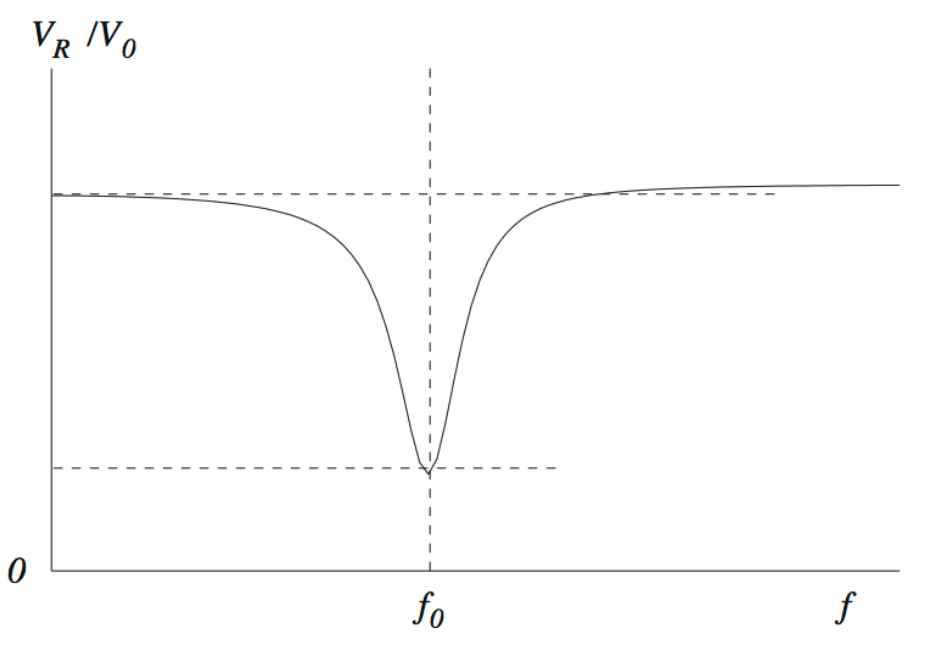
\includegraphics[width=.65\textwidth]{ParallelResonanceCurve.png}
           \caption{Parallel Resonance Curve}
           \label{fig:Parallel Resonance Curve}
        \end{center}
    \end{figure}
    We'll discuss this more in the following section.

    \section{The Series Resonance LRC Circuit}\label{sec:Series Resonance}
    In this set-up we have all three components, the inductor, capacitor, and resistor, in series, as 
    below.
    \begin{figure}[H]
        \centering
            \def\svgwidth{0.5\textwidth}
            \input{SeriesResonanceCircuit.pdf_tex}
            \caption{Series Resonance Circuit}
            \label{fig:Series Resonance Circuit}
    \end{figure}
    As you might imagine, the transfer function for this configuration is slightly different to 
    \autoref{eqn:Parallel Transfer Function}. In fact we will derive it now. \newline \newline
    We begin with the definition of the transfer function:
    \begin{equation*}
        H(\omega)=\frac{V_{out}}{V_{in}}
    \end{equation*}
    where $V_{in}$ is the voltage supplied by our AC source and $V_{out}$ is the voltage drop across 
    the resistor, which we know will be 
    \begin{equation*}
        V_{out}=iR
    \end{equation*}
    but as this is a series circuit we know that the current in all the components will always be the 
    same value
    \begin{equation*}
        i=\frac{V_{in}}{|Z(\omega)|}
    \end{equation*}
    where $Z(\omega)$ is the impedance of this circuit. Again this is a series circuit so the total 
    impedance is merely the sum of the impedance of the respective components.
    \begin{align*}
        Z(\omega)&=Z_L+Z_C+Z_R\\
        &=(0+jL\omega)+(0-j\frac{1}{C\omega})+(R+0j)\\
        &=R+j(L\omega-\frac{1}{C\omega})
    \end{align*}
    where we're using $j$ as the imaginary unit. Current is not complex, which is why we have $|Z|$ 
    previously. We can calculate this value
    \begin{align*}
        |Z(\omega)|&=\sqrt{Z\cdot Z*}\\
        &=\sqrt{(R+j(L\omega-\frac{1}{C\omega}))(R-j(L\omega-\frac{1}{C\omega}))}\\
        &=\sqrt{R^2+(L\omega-\frac{1}{C\omega})^2}\\
        &=\sqrt{R^2+L^2\omega^2-2\frac{L}{C}+\frac{1}{C^2\omega^2}}\\
        &=\frac{1}{C\omega}\sqrt{C^2\omega^2R^2+L^2C^2\omega^4-2LC\omega^2+1}\\
        &=\frac{1}{C\omega}\sqrt{(C\omega R)^2+(1-LC\omega^2)^2}
    \end{align*}
    Which means that we have 
    \begin{align*}
        i&=\frac{V_{in}}{\frac{1}{C\omega}\sqrt{(C\omega R)^2+(1-LC\omega^2)^2}}\\
        &=\frac{V_{in}C\omega}{\sqrt{(C\omega R)^2+(1-LC\omega^2)^2}}\\
        \implies V_{out}&=\frac{RV_{in}C\omega}{\sqrt{(C\omega R)^2+(1-LC\omega^2)^2}}\\
        \implies H(\omega)&=\frac{RV_{in}C\omega}{V_{in}\sqrt{(C\omega R)^2+(1-LC\omega^2)^2}}
    \end{align*}
    So we have our transfer function for the series resonance circuit:
    \begin{equation}
        H(\omega)=\frac{RC\omega}{\sqrt{(C\omega R)^2+(1-LC\omega^2)^2}}
        \label{eqn:Series Transfer Function}
    \end{equation}
    This equation has the same extremum as the parallel circuit, except it has a maximum at 
    $\omega_0=\frac{1}{\sqrt{LC}}$ rather than a minimum. Plotting this function we did in 
    \autoref{fig:Parallel Resonance Curve} we get 
    \begin{figure}[H]
        \begin{center}
           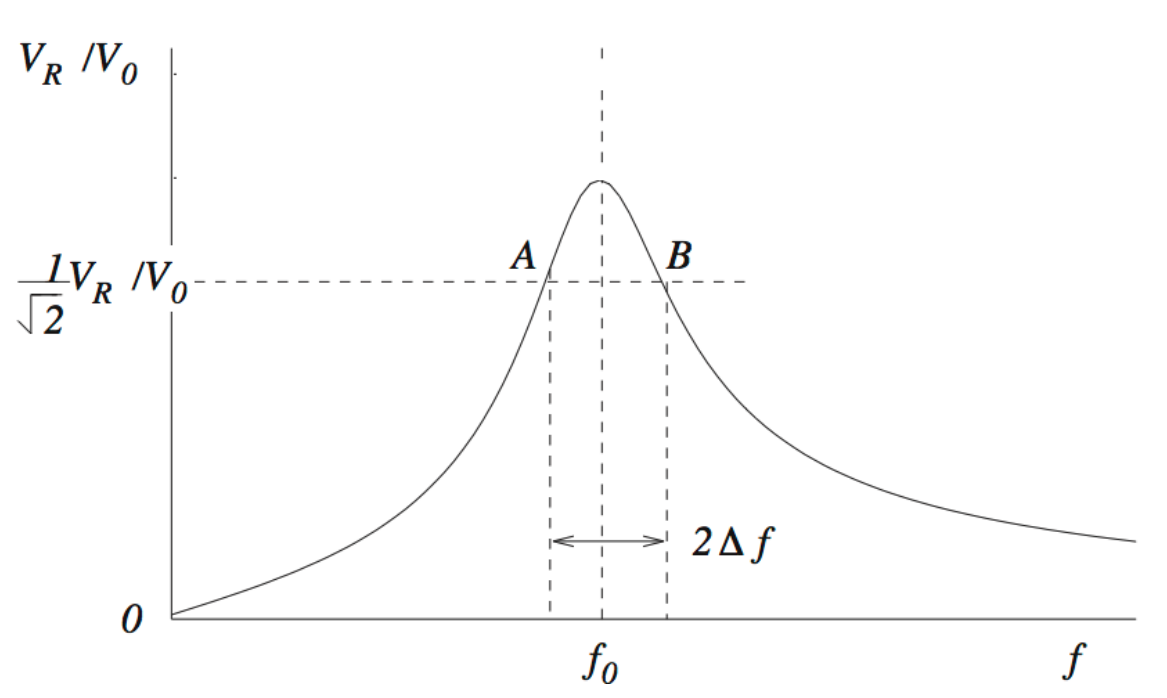
\includegraphics[width=.65\textwidth]{SeriesResonanceCurve.png}
           \caption{Series Resonance Curve}
           \label{fig:Series Resonance Curve}
        \end{center}
    \end{figure}
    These plots have $f$ along the horizontal axis as that's the input frequency but that is no problem 
    as $f=\frac{\omega}{2\pi}$. From the values of $2\Delta f$ and $f_0$ we can define a parameter 
    we call the quality factor 
    \begin{equation*}
        Q=\frac{f_0}{2\Delta f}=\frac{\omega_0L}{R}
        \label{eqn:Quality Factor}
    \end{equation*}
    that describes the "sharpness" of this curve, the larger $Q$ is, the sharper the curve. From 
    \autoref{eqn:Quality Factor} we see that the resistance and inductance in the circuit has an 
    impact on $Q$ and thus on the shape of the resonance curve. Note that this quality factor and its 
    associated usefulness is not unique to the series resonance circuit, it applies to the parallel 
    circuit too and we will use this in later sections to analyse specific circuits.

    \section{Experiment}\label{sec:Experiment}
    In the experimental section of this report we will be investigating the behaviour of both the 
    parallel and series resonance circuits by way of setting them up on a breadboard to see how they 
    behave in reality, as well as using a simulation of each. 
    \subsection{Apparatus}
    We used the following items, all with standard measurement uncertainty of 2\%:
    \begin{itemize}
        \item 1 1 k$\Omega$ resistor (actual measured value 984.4 $\Omega$).
        \item 2 100 $\Omega$ resistors (actual measured value 98.0 and 98.6 $\Omega$).
        \item 1 96.51 nF capacitor (actual measured value 93.94 nF).
        \item 1 70 mH inductor (actual measured value 73.62 mH).
        \item 1 myDAQ.
        \item 1 screwdriver.
        \item 1 function generator.
        \item 1 digital oscilloscope.
        \item 1 breadboard.
        \item Wire (with negligible resistance).
    \end{itemize}
    Our parallel circuit was set up with the 1 k$\Omega$ resistor and the series circuit was set up 
    with the two 100 $\Omega$ resistors in series to achieve a total resistance of 200 $\Omega$. 
    They were set up in the same configuration as in \autoref{fig:Parallel Resonance Circuit} and 
    \autoref{fig:Series Resonance Circuit}. 

    \subsection{Method}
    To collect our data (thanks Prof Blumenthal) we started off using the function generator to apply 
    a sinusoidal alternating voltage across the parallel and series circuits with the oscilloscope 
    measuring the voltage across the resistor. By adjusting the frequency of the function generator 
    we were able to find the point at which the voltage across the resistor was minimised or maximised, 
    depending on the type of circuit. The oscilloscope displays for each circuit are pictured 
    in \autoref{fig:Parallel Resonance Scope} and \autoref{fig:Series Resonance Scope}
    \begin{figure}[h]
        \begin{center}
           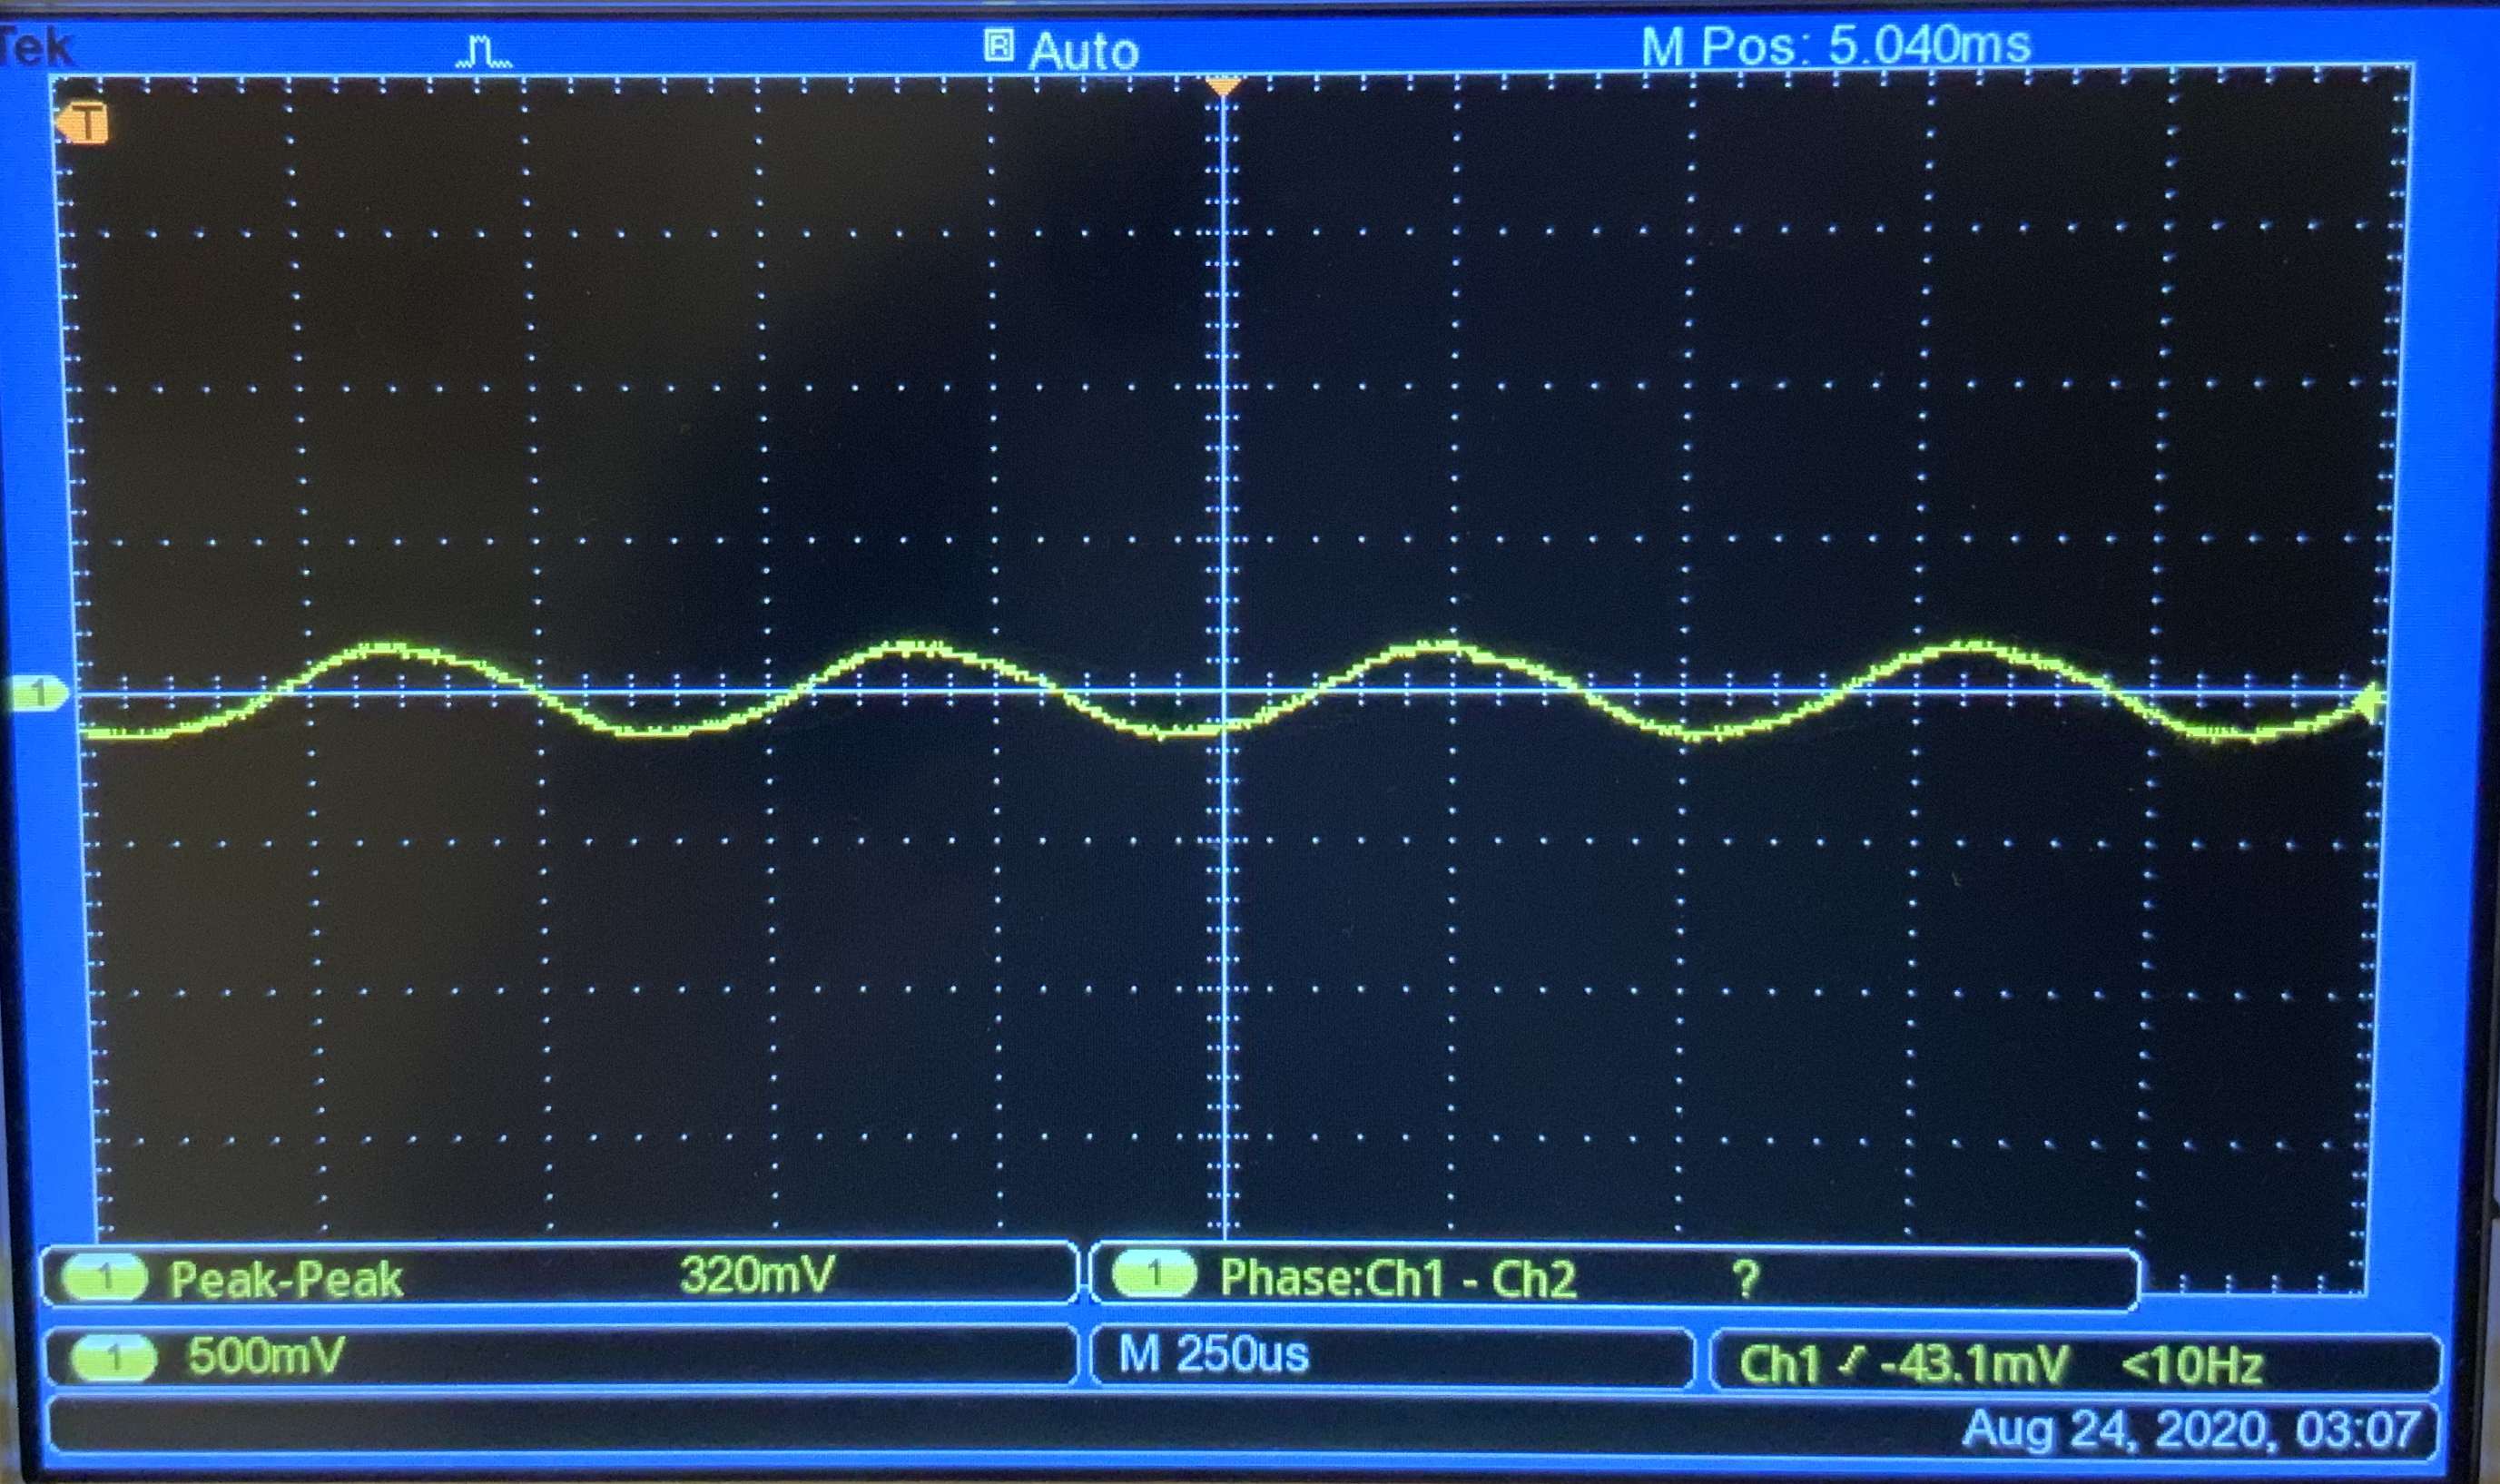
\includegraphics[width=.65\textwidth]{Parallel_Resonance_Scope.jpg}
           \caption{Parallel Resonance Circuit at resonance}
           \label{fig:Parallel Resonance Scope}
        \end{center}
    \end{figure}
    \begin{figure}[h]
        \begin{center}
           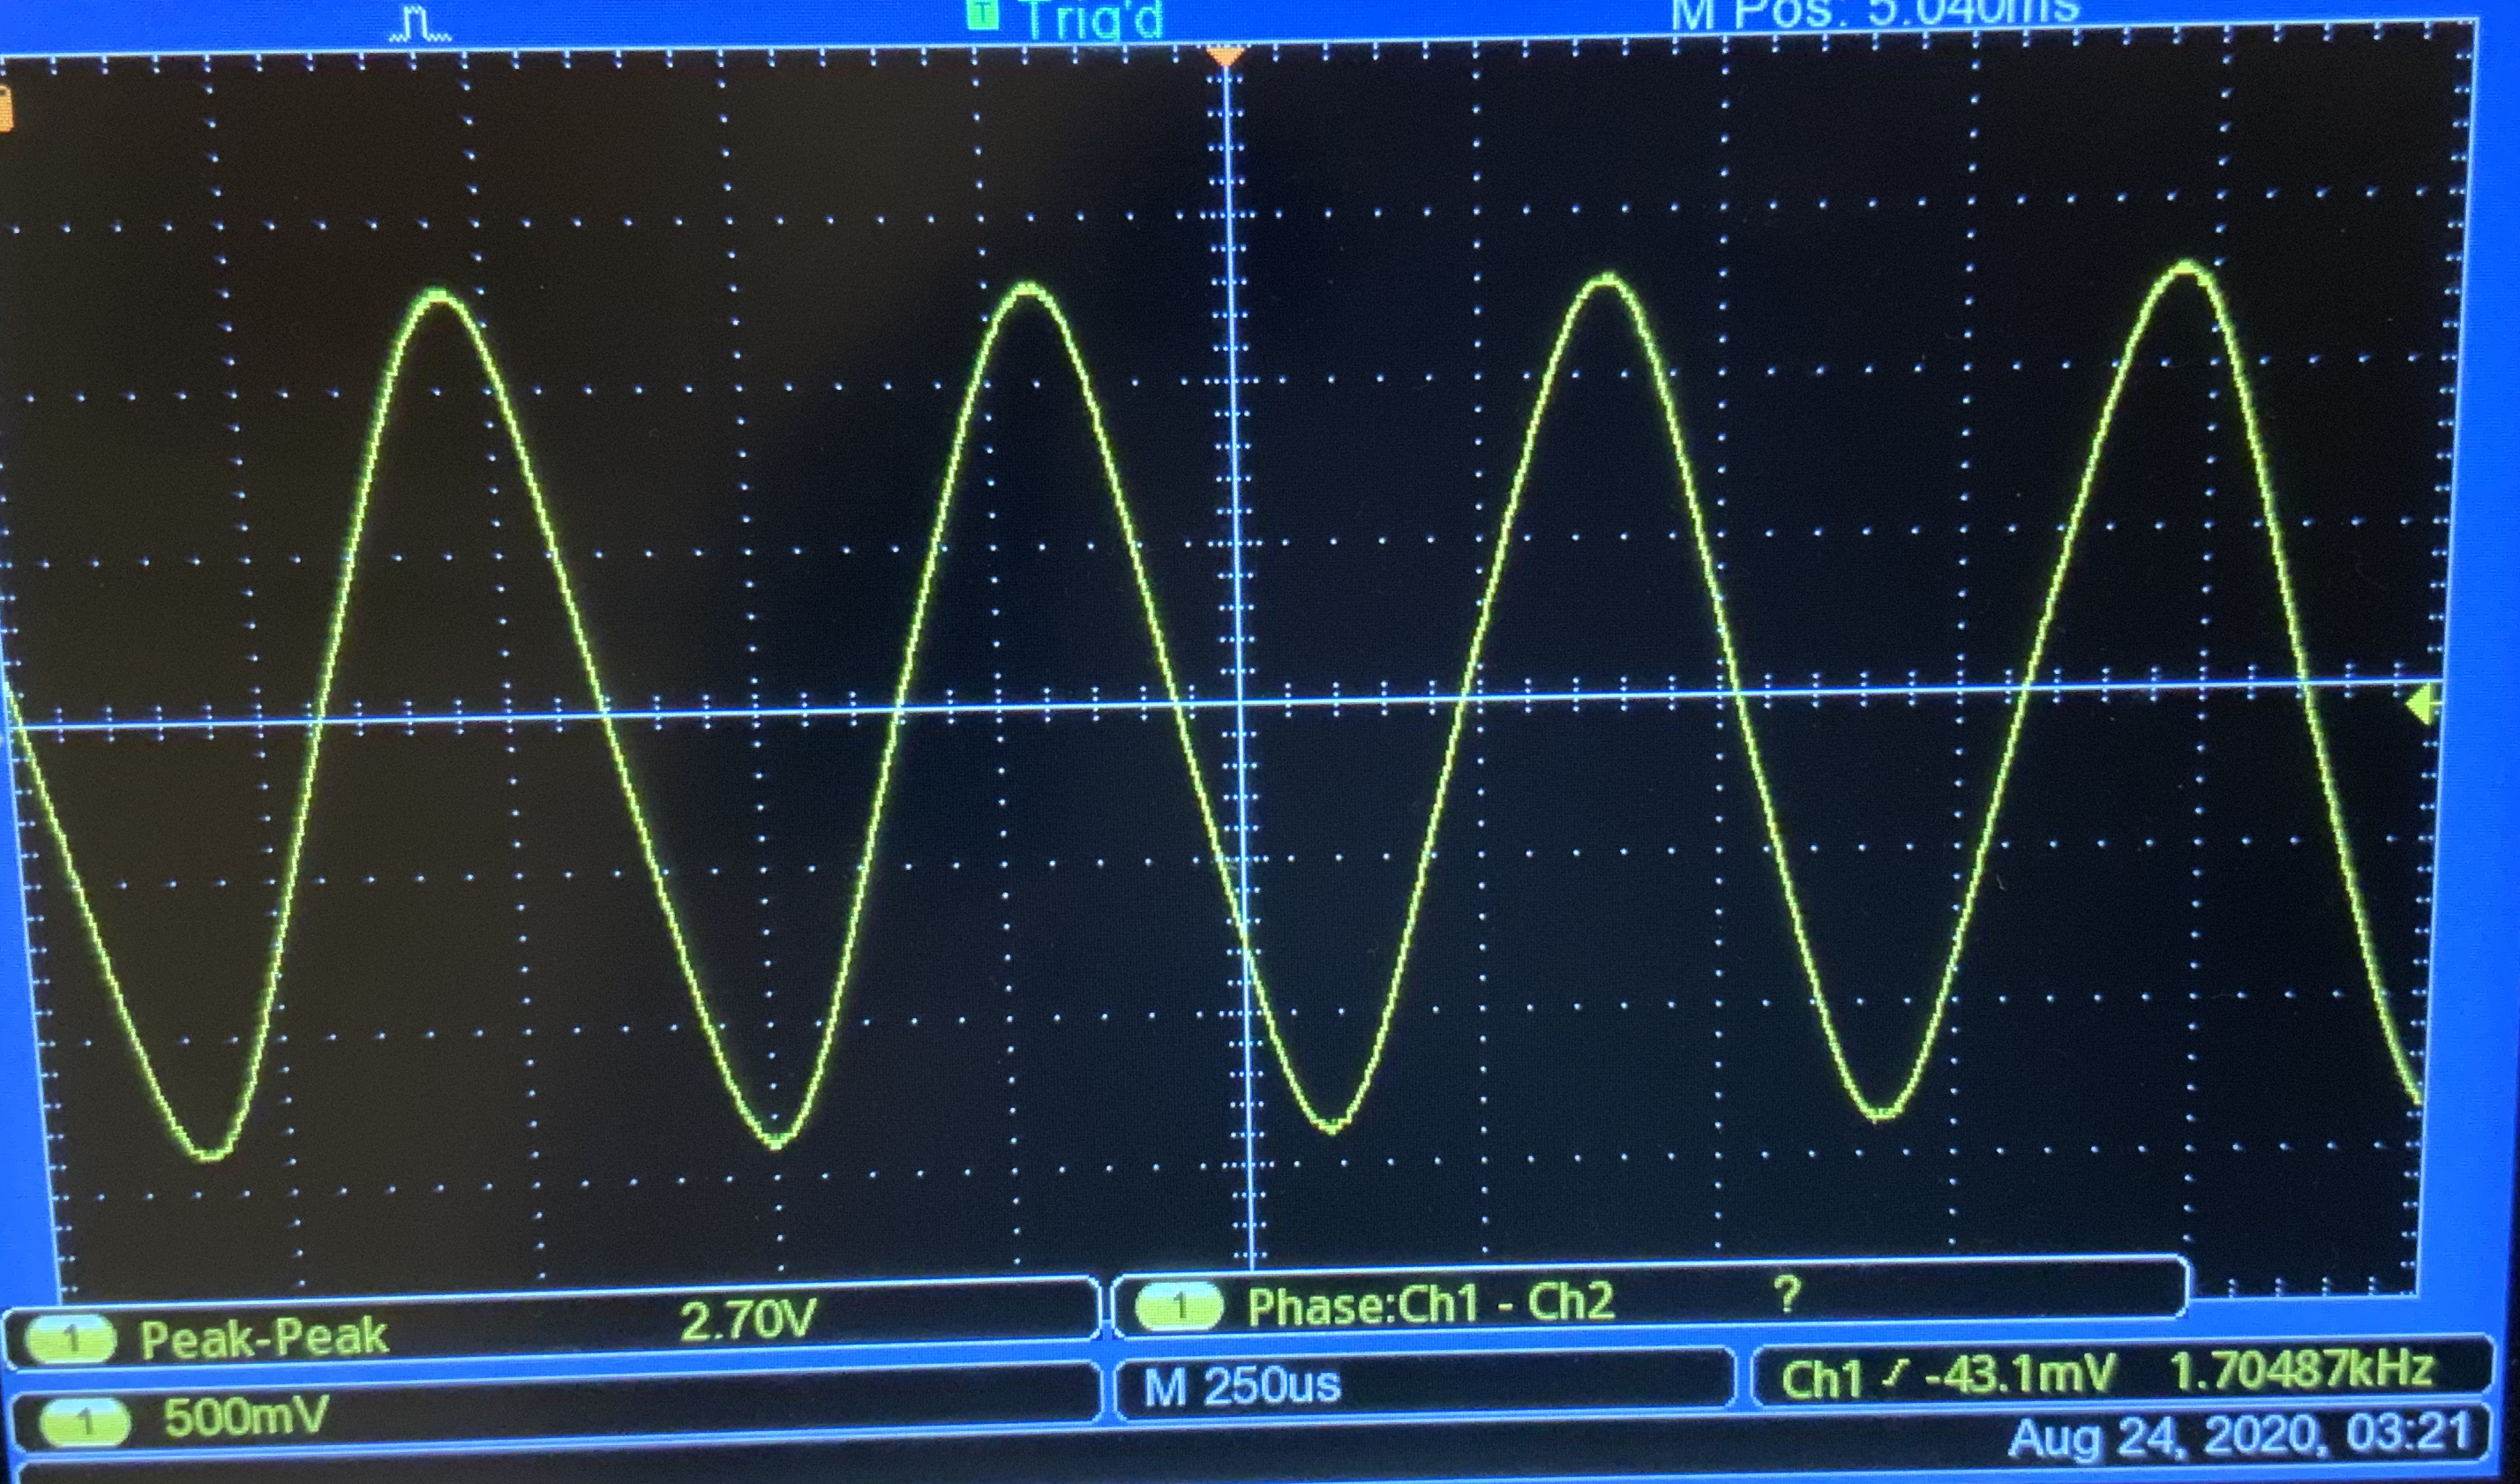
\includegraphics[width=.65\textwidth]{Series_Resonance_Scope.jpg}
           \caption{Series Resonance Circuit at resonance}
           \label{fig:Series Resonance Scope}
        \end{center}
    \end{figure}
    Next we used the \texttt{LCsim.exe} program to simulate the parallel and series circuits with 
    a range of different resistance values to investigate how the value of R affects the value of $Q$. 
    
    
\end{document}